\chapter{Models}
\label{sec:models}

This chapter explores different probabilistic models for the problem, explains how they can be efficiently learned from data and presents the learning algorithm's performance on synthetic data.

\section{Submodular model: FLID}

The Facility Location Diversity (FLID) model was first proposed by \citet{tschiatschek16learning} and belongs to the class of log-submodular probability distributions over sets.

\begin{definition}
  A distribution over sets $S \subseteq V$, where w.l.o.g $V = \{1,\dots,|V|\}$, of the form $P(S) = \frac{1}{Z}\mathrm{exp}(F(S))$ is called a log-submodular probability distribution, if $F(S)$ is a submodular function \citep{djolonga14variational}.
\end{definition}

\begin{definition}
  \label{def:submodularity}
  A function $F:2^V \rightarrow \mathbb{R}$ is submodular if it exhibits a "diminishing returns" property \citep{krause14submodular}, namely:
    \begin{equation*}
      \forall S,T \subseteq V : S \subseteq T, i \notin T \mid F(S \cup i) - F(S) \geq F(T \cup i) - F(T)
    \end{equation*}
\end{definition}

Submodular functions intuitively indicate that adding an item to a smaller set results in a larger gain than adding it to a larger one. This is a natural property in the context of summarization where adding more information to a large summary is less effective than adding it to a smaller one.

The FLID model consists of two terms, a modular one which considers the individual utility or relevance of the items in the set, namely:

\begin{equation}
  \label{eq:modular}
  P(S) \propto \exp\left(\sum_{i \in S}u_{i}\right)
\end{equation}

Where $u_{i} \in \mathbb{R}$ quantifies the utility of item $i$. In the context of location summarization, this utility could be proportional to the popularity of a place or how many times it has been photographed.

The diversity term is based on the idea of a latent concept space of dimension $L$ where each item can be represented with a vector $\mathbf{w}^{b}_{i} \in \mathbb{R}^{L}_{\geq 0}$. The representation in this space allows the model to identify items that are similar and penalize sets that include them together. Formally, the diversity term for a set $S \subseteq V$ is:

\begin{equation}
  \label{eq:diversity}
  \mathrm{div}(S) = \sum_{d=1}^{L}\left(\max_{i \in S}{w^{b}_{i, d}} - \sum_{i \in S}{w^{b}_{i,d}}\right)
\end{equation}

Putting this two terms together results in the \ref{eq:flid} probability model proposed by \citet{tschiatschek16learning}.

\begin{equation}
  \tag{FLID}
  P(S) = \frac{1}{Z}\exp{\left(\sum_{i \in S}u_{i} + \sum_{d=1}^{L}\left(\max_{i \in S}{w^{b}_{i, d}} - \sum_{i \in S}{w^{b}_{i,d}}\right)\right)}
  \label{eq:flid}
\end{equation}

In this model, $\mathbf{u} \in \mathbb{R}^{|V|}$ is the vector of utilities and $\mathbf{W}^{b} \in \mathbb{R}_{\geq 0}^{|V| \times L}$ is the diversity weight matrix where each row is the aforementioned $\mathbf{w}^{b}_{i}$ vector. $u_{i}$ is the $i$-th entry of $\mathbf{u}$ and $w^{b}_{i,d}$ is the $(i,d)$-th entry of $\mathbf{W}^{b}$. The positivity constraint on $\mathbf{W}^{b}$ is required to ensure that the model is log-submodular.

\subsection{Partition function}

In log-submodular probabilistic models, the normalization constant $Z$ is known as the \textit{partition function} \citep{djolonga14variational} and its exact computation is known to be \#P-complete \citep{jerrum1990}.  However, it has been proven that for FLID the partition function can be computed exactly in $\mathcal{O}(|V|^{L+1})$ time, which can be efficient for $L \ll |V|$ \citep{tschiatschek16learning}. This is an important property because the partition function is necessary to compute marginal probabilities and other quantities from the model.

\subsection{Example: Two landmarks}
\label{sec:flid-toy}

In order to illustrate the model, consider a town with 3 popular locations: A town hall ($h$), a statue ($s$) and a fountain ($f$). Data shows that visitors only take photos at either the town hall and the statue, or at the town hall and the fountain. This can be modeled with FLID by introducing a latent concept that discourages taking photos at both the fountain and statue.

Concretely, let $V = \{h, s, f\}$ and $\mathbf{u} = \left(2, 2, 2\right)^{\intercal}$, indicating that all locations are equally popular. A suitable diversity weight vector would then be $\mathbf{W}^{b} = \left(0, 20, 20\right)^{\intercal}$. Table \ref{tab:flid-toy-probs} shows the resulting probabilities of the subsets, accurately representing the aforementioned description of the problem. Note that the probabilities are not exactly $\nicefrac{0.5}{0.5}$ for the sets of interest but this can be easily fixed by increasing the utilities to ensure that sets of size 2 have a larger unnormalized magnitude compared to individual ones.

\begin{table}
  \centering
  \caption{FLID probability distribution for the scenario in example \ref{sec:flid-toy}}
  \begin{tabular}{@{}ll@{}}
    \toprule
      $S$ & $P(S)$  \\
    \midrule
      $\{h,s\}, \{h,f\}$ & $\approx 0.41$ \\
      $\{h\}, \{s\}, \{f\}$ & $\approx 0.06$ \\
      $\{\}, \{s,f\}, \{h,s,f\}$ & $\approx 0.00$ \\
    \bottomrule
  \end{tabular}
  \label{tab:flid-toy-probs}
\end{table}

\section{Mixed model: FLDC}

Diversity is an important property in the context of summarization \citep{tschiatschek16learning}, however coherence is also a desired property of summaries \citep{Yan:2011:ETS:2009916.2010016}. Balancing coherence and diversity is considered a challenge because maxiziming only one of these properties may lead to poor results on the other one \citep{Shahaf2012}.

In order to model coherence in this model, the addition of a log-supermodular term analogous to the diversity term \ref{eq:diversity} is proposed.

\begin{definition}
  \label{def:supermodularity}
  A function $F:2^V \rightarrow \mathbb{R}$ is supermodular iff $-F(S)$ is submodular.
\end{definition}

The supermodular term encodes the items into another latent concept space, of dimension $K$, where sets containing items with high values in some latent dimension are rewarded. Hence modeling complementarity between items.

For example, consider a spatial summary of a city where people tend to stay close to the city center. A possible latent dimension could encode the distance to the center, and rewarding coherence on this dimension would create summarizes where all locations are close together which is the modeled behavior.

The extended model will be reffered to as the Facility Location Diversity and Coherence (\ref{eq:fldc}) model and its probability distribution is given by:

\begin{equation}
  \tag{FLDC}
  P(S) = \frac{1}{Z}\exp{\left(\sum_{i \in S}{u_{i}} + \mathrm{div}(S) + \sum_{c=1}^{K}{\left(\sum_{i \in S}{w^{e}_{i,c}} - \max_{i \in S}{w^{e}_{i,c}}\right)}\right)}
  \label{eq:fldc}
\end{equation}

Where $w^{e}_{i,c}$ is the $(i,c)$-th entry of $\mathbf{W}^{e}$. Each row of $\mathbf{W}^{e}$ encodes the representation of an item $i$ in the newly introduced concept space of dimension $K$, hence $\mathbf{W}^{e} \in \mathbb{R}^{|V|\times K}_{\geq 0}$. Once again a positivity constraint is introduced, in this case to ensure the term is a supermodular function.

It should be noted that the FLDC model is neither log-submodular or log-supermodular unless $K=0$ or $L=0$, respectively. However, it can be used and learned in a similar fashion as the FLID model.

\subsection{Example: Disjoint pairs}
\label{sec:fldc-toy}

As an example of the extended model, consider the distribution presented in table \ref{tab:fldc-toy-probs} for $V = \{1,2,3,4\}$. It represents a set of two disjoint pairs, which indicates there exists a diversity component between the two pairs whilist having a coherence component between the items contained in each pair.

Concretely, the weight matrices $\mathbf{W}^{b}, \mathbf{W}^{e}$ in figure \ref{fig:fldc-toy-mixed-weights} illustrate one possible instance of the model. The corresponding utility vector is $\mathbf{u} = \overrightarrow{0}$, because there is no indication that individual items are favored over the pairs. Note that this model is easily interpretable and accurately realizes the distribution.

\begin{table}
  \centering
  \caption{Probability distribution for example \ref{sec:fldc-toy}}
  \begin{tabular}{@{}ll@{}}
    \toprule
    $S$ & $P(S)$  \\
    \midrule
    $\{1,2\}, \{3,4\}$ & $0.5$ \\
    $2^V \setminus \{\{1,2\}, \{3,4\}\}$ & $0.0$ \\
    \bottomrule
  \end{tabular}
  \label{tab:fldc-toy-probs}
\end{table}

\begin{figure}
  \centering
  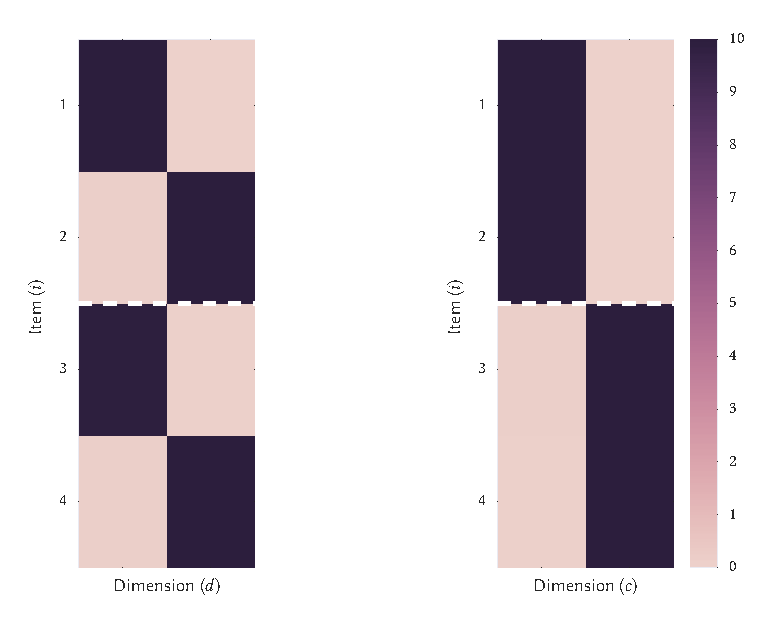
\includegraphics[width=\textwidth]{fldc_toy_example_mixed_weights}
  \caption{Diversity and coherence weights for FLDC model in example \ref{sec:fldc-toy}. The dotted line divides the paired items.}
  \label{fig:fldc-toy-mixed-weights}
\end{figure}

\section{Featurized model: FFLDC}

An important characteristic of the FLDC and FLID models is that they are agnostic to the type of items in the ground set, this allows its application to a wide range of problems without prior knowledge. However the downside is that the model has no capability to make use of information about the items, if available, to improve the modeling of the data. Moreover, if a new item is added to the set there is no way to generalize the existing knowledge about similar items to it.

In order to solve these problems, a further extension to the model is proposed. Firstly, the information about each item ($i \in V$) is represented as a vector $\mathbf{x}_{i} \in \mathbb{R}^{M}$ where each entry is a feature, e.g. for venues one feature could be its aggregated rating while another indicates whether it is indoors or outdoors.

Then, the utility vector $\mathbf{u}$ and weight matrices $\mathbf{W}^{b}, \mathbf{W}^{e}$ are factorized to include the feature matrix $\mathbf{X} \in \mathbb{R}^{|V| \times M}$ as follows:

\begin{align}
  \mathbf{u} &= \mathbf{Xa}   \label{eq:ffldc-factorization-1} \\
  \mathbf{W}^{b} &= \mathbf{XB}  \label{eq:ffldc-factorization-2} \\
  \mathbf{W}^{e} &= \mathbf{XE}
  \label{eq:ffldc-factorization-3}
\end{align} 

Where $a \in \mathbb{R}^{M}$ represents the contribution of each feature to the total utility of an item, whilist $\mathbf{B} \in \mathbb{R}^{M \times L}$ and $\mathbf{E} \in \mathbb{R}^{M \times K}$ encode the contribution of each feature to each latent diversity and coherence dimension, respectively. The intuition behind this factorization is that the information about the items can enhance the latent representations, hence producing a richer model.

The extended model will be reffered to as the Featurized Facility Location Diversity and Coherence (FFLDC) model and its probability distribution is given by:

\begin{align}
  \tag{FFLDC} \label{eq:ffldc}
  P(S) &= \frac{1}{Z}\exp{\left(\sum_{i \in S}{\sum_{k=1}^{M}x_{i,k}a_{k}} + fdiv(S) + fcoh(S)\right)} \\
  fdiv(S) &= \sum_{d=1}^{L}{\left(\max_{i \in S}{\sum_{k=1}^{M}x_{i,k}b_{k,d}} - \sum_{i \in S}{\sum_{k=1}^{M}x_{i,k}b_{k,d}}\right)} \\
  fcoh(S) &= \sum_{c=1}^{K}{\left(\sum_{i \in S}{\sum_{k=1}^{M}x_{i,k}e_{k,c}} - \max_{i \in S}{\sum_{k=1}^{M}x_{i,k}e_{k,c}}\right)}
\end{align}

Where $a_{i}$ is the $i$-th entry of $\mathbf{a}$, $b_{k,d}$ is the $(k,d)$-th entry of $\mathbf{B}$, $e_{k,d}$ is the $(k,e)$-th entry of $\mathbf{E}$ and $x_{i,k}$ is the $(i,k)$-th entry of $X$.

\begin{remark}
  If $\mathbf{X} = \mathcal{I}$, then FFLDC is equivalent to FLDC, with $\mathbf{a} = \mathbf{u}$, $\mathbf{W}^{b} = \mathbf{B}$ and $\mathbf{W}^{e} = \mathbf{E}$.
\end{remark}

The use of features also allows the application of the model to previously unknown items, hence solving the aforementioned problem of generalization. This is because the parameters of the FFLDC model, i.e. $\mathbf{a}, \mathbf{B}, \mathbf{E}$, do not depend on the ground set $V$ but rather on the space of features $\mathbb{R}^{M}$. If an item $j \notin V$ is considered, a model learned on only items in $V$ can immediately be applied to the new set $V \cup \{j\}$ using only its feature representation, contrary to the case of FLID or FLDC where it would require adding a new row to the weight matrices and learning it.

\subsection{Example: Rated locations}
\label{sec:ffldc-toy}

A simple town has 6 popular locations, each of them has been rated from 0 (terrible) to 5 (excellent). It is known that a typical visitor cares about these ratings but also is interested in visiting places that are outdoors and/or serve food. Given data from previous visitors, shown in table \ref{tab:ffldc-toy-probs}, the task is to model this behavior using the FFLDC model.

\begin{table}
  \centering
  \caption{Synthetic data for example \ref{sec:ffldc-toy}}
  \begin{tabular}{@{}ll@{}}
    \toprule
    Locations visited $(S)$ & $P(S)$  \\
    \midrule
    $\{1,3\}$ & $0.30$ \\
    $\{3,4\}$ & $0.25$ \\
    $\{3,6\}$ & $0.15$ \\
    $\{2\}$ & $0.10$ \\
    $\{1\}$ & $0.06$ \\
    $\{3\}, \{4\}$ & $0.04$ \\
    $\{5\}, \{6\}$ & $0.03$ \\
    \bottomrule
  \end{tabular}
  \label{tab:ffldc-toy-probs}
\end{table}

In this example there is knowledge about the items and what features are relevant for the data. These features are summarized in equation \ref{eq:ffldc-toy-feats}. The first column corresponds to the aforementioned rating, the second and third are binary features indicating whether the location is an outdoor one and whether it serves food, respectively.

\begin{equation}
  \mathbf{X} = \left(
    \begin{array}{ccc}
      4 & 1 & 0 \\
      4 & 1 & 1 \\
      3 & 0 & 1 \\
      3 & 1 & 0 \\
      2 & 1 & 1 \\
      2 & 1 & 0  \\
     \end{array}
  \right)
  \label{eq:ffldc-toy-feats}
\end{equation}

Looking at the data and features, it is possible to draw a FFLDC model that encourages diversity on the second a third feature while assigning a positive utility and coherence values to the first feature. One such model is presented in figure \ref{fig:ffldc-toy-all-weights}, this approximates distribution from table \ref{tab:ffldc-toy-probs} and illustrates the type of model that is useful in this example.

\begin{figure}
  \centering
  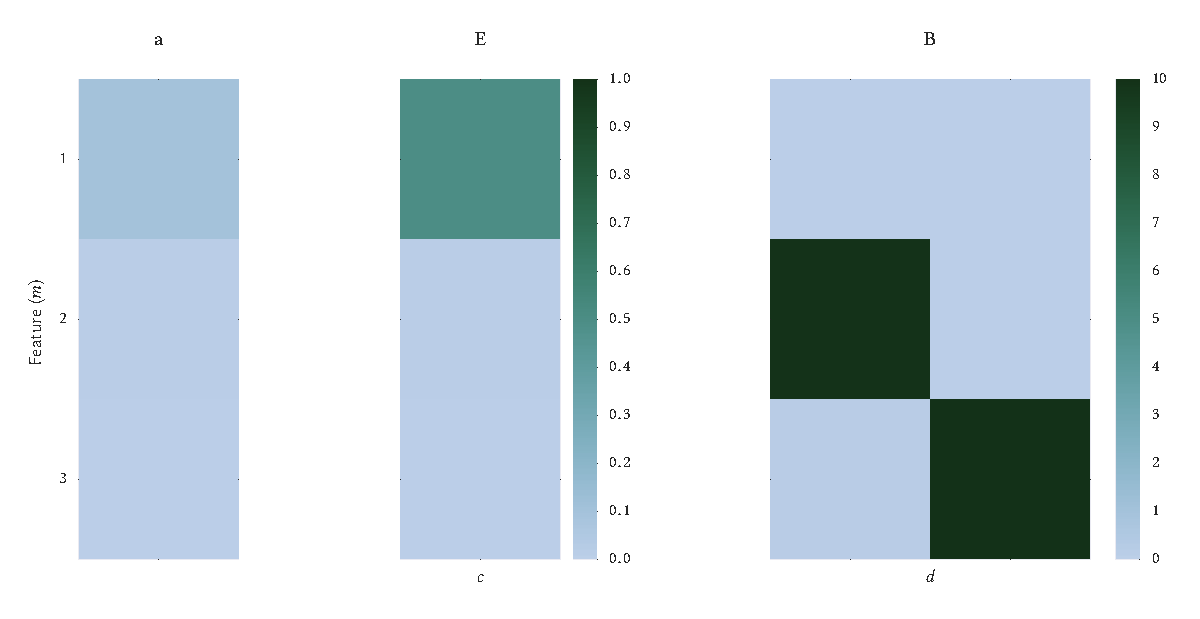
\includegraphics[width=\textwidth]{ffldc_toy_example}
  \caption{FFLDC sample model for example \ref{sec:ffldc-toy}.}
  \label{fig:ffldc-toy-all-weights}
\end{figure}

With this model, if a new location $j$ is considered then it is straightforward to estimate what its probability of being visited $P(j \in S)$ would be, only knowing its feature representation.

\section{Learning from data}

As noted by \citet{tschiatschek16learning}, Maximum Likelihood Estimation (MLE) is generally intractable in FLID due to the complexity of computing the partition function for large $L$. This result can be extended to the FLDC model utilizing the fact that the algorithm presented by \citet{tschiatschek16learning} for computing $Z$ doesn't require the diversity weights $w^{b}_{i,d}$ to be positive, therefore it can be easily extended to included the coherence weights as negative diversity ones.

\begin{proposition}
  The time complexity of calculating the partition function for the FLDC model is $\mathcal{O}(|V|^{L+K+1})$, using a modified version of the algorithm proposed by \citep{tschiatschek16learning}.
\end{proposition}

Additionally, this result can be extended to the FFLDC case because a FFLDC model can always be reduced to an equivalent FLDC model through the factorization in equations \ref{eq:ffldc-factorization-1}-\ref{eq:ffldc-factorization-3}. This reduction has a time complexity of $O(M|V|(L+K))$, corresponding to the matrix multiplications, which is considerably smaller than the complexity of the partition function computation for FLDC.

Fortunately, there exists an alternative method for estimating unnormalized probabilistic models from observed data, i.e. without computing the partition function. This method is called Noise Constrastive Estimation (NCE) \citep{Gutmann12NCE} and it will be described in more detail in the following section.

\subsection{NCE Learning}

The idea behind NCE is to transform the unsupervised learning task of estimating a probability density from data into a supervised classification task. In order to do this, the observed data $\mathcal{D}$, assumed to be drawn from an unknown distribution $P_{d}$, is compared to an artificially generated set of noise samples $\mathcal{N}$ drawn from a known distribution $P_{n}$. The classification task is then setup to optimize the likelihood of correctly discriminating each sample as either observed data or artificial noise.

Formally, denote $\mathcal{A}$ as the complete set of labeled samples, i.e. $\mathcal{A} = \{(S,Y_{s}) : S \in \mathcal{D} \cup \mathcal{N}\}$ where $Y_{s} = 1 \equiv S \in \mathcal{D}$ and $Y_{s} = 0 \equiv S \in \mathcal{N}$. Additionally, let $\nu$ be the noise-to-data ratio, i.e. $\nu = \nicefrac{|\mathcal{N}|}{|\mathcal{D}|}$.

The goal is to estimate the posterior probabilities $P(Y_{s} = 1 \mid S;\theta)$ and $P(Y_{s} = 0 \mid S;\theta)$, in order to discriminate noise from data samples. These probabilities are given by equations \ref{eq:posterior-1} and \ref{eq:posterior-2}.

\begin{align}
  P(Y_{s} &= 1 \mid S;\theta) = \frac{\hat{P}_{d}(S;\theta)}{\hat{P}_{d}(S;\theta) + \nu P_{n}(S)}
  \label{eq:posterior-1} \\
  P(Y_{s} &= 0 \mid S;\theta) = \frac{\nu P_{n}(S)}{\hat{P}_{d}(S;\theta) + \nu P_{n}(S)}
  \label{eq:posterior-2}
\end{align}

It is worth noting that a estimated distribution $\hat{P}_{d}$ is used instead of $P_{d}$, because the real density is not known. As indicated by \citet{Gutmann12NCE}, $\hat{P}_{d}$ can be an unnormalized distribution for NCE where the partition function $Z$ is included in the set of parameters $\theta$ as $\hat{Z}$, hence resulting in an approximately normalized distribution after the optimization.

Estimating the posterior probabilities is equivalent to maximizing the conditional log-likelihood objective in \ref{eq:log-likelihood} \citep{Gutmann12NCE}.

\begin{equation}
  \label{eq:log-likelihood}
  g(\theta) = \sum_{S \in \mathcal{D}}{\log{P(Y_{s} = 1 \mid S;\theta)}} + \sum_{S \in \mathcal{N}}{\log{P(Y_{s} = 0 \mid S;\theta)}}
\end{equation}

For the models previously introduced, the set of parameters $\theta$ to adjust in order to maximize the objective are:

\begin{itemize}
  \item FLID \citep{tschiatschek16learning}: $\theta = [\hat{Z}, \mathbf{u}, \mathbf{W}^{b}]$.
  \item FLDC: $\theta = [\hat{Z}, \mathbf{u}, \mathbf{W}^{b}, \mathbf{W}^{e}]$.
  \item FFLDC: $\theta = [\hat{Z}, \mathbf{a}, \mathbf{B}, \mathbf{E}]$.
\end{itemize}

Lastly, a couple of conditions must be taken into consideration for NCE to work \citep{Gutmann12NCE}:

\begin{enumerate}
  \item The parameterized probability function $\hat{P}_{d}(S;\theta)$ must be of the same family as the real distribution $P_{d}$, i.e. $\exists \theta^{*} \mid \hat{P}_{d}(S;\theta^{*}) = P_{d}$.
  \item The noise distribution $P_{n}$ is nonzero whenever $P_{d}$ is nonzero.
\end{enumerate}

Stochastic Gradient Descent (SGD) will be used for the training of the proposed models, this is the same method used by \citet{tschiatschek16learning} for the FLID model. SGD is a gradient-based method that has proven effective in large-scale learning tasks due to its efficiency when the computation time is a limiting factor \citep{Bottou2010, Zhang2004}, hence making it appropriate for the scale of data sourced from the internet, such as public user photos in Flickr.

In each iteration, the sub-gradient $\nabla \log{P(Y_{s} = y \mid S;\theta)}$ must be computed. The following sections define the sub-gradient for each model.

\subsubsection{FLID}

For FLID, $\nabla \log{P(Y_{s} = y \mid S;\theta)}$ is given by the following equations \citep{tschiatschek16learning}:

\begin{align}
  \nabla \log{P(Y_{s} = y \mid S;\theta)} &= \left(y - \frac{1}{1 + \nu \frac{P_{n}(S)}{\hat{P}_{d}(S;\theta)}}\right) \nabla \log{\hat{P}_{d}(S;\theta)} \\
  \hat{P}_{d}(S;\theta) &= \frac{1}{\hat{Z}}P(S; \mathbf{u}, \mathbf{W}^{b}) \\
  \left(\nabla_{\mathbf{u}}\log{\hat{P}_{d}(S; \hat{Z}, \mathbf{u}, \mathbf{W}^{b})}\right)_{i} &= \begin{cases}
  1 &  \text{if}\ i \in S \\
  0 & \text{otherwise}
  \end{cases} \\
  \left(\nabla_{\mathbf{W}^{b}}\log{\hat{P}_{d}(S; \hat{Z}, \mathbf{u}, \mathbf{W}^{b})}\right)_{i,d} &= \begin{cases}
    -1 & \text{if}\ i \in S\ \text{and}\ i \neq \argmax_{j \in S}{w^{b}_{j,d}} \\
     0 & \text{otherwise}
  \end{cases} \\
  \nabla_{\hat{Z}}\log{\hat{P}_{d}(S; \hat{Z}, \mathbf{u}, \mathbf{W}^{b})}&= \frac{-1}{\hat{Z}}
\end{align}

Where $P(S;\mathbf{u}, \mathbf{W}^{b})$ is the unnormalized \ref{eq:flid} equation, $\left(\nabla_{\mathbf{u}}\cdot \right)_{i}$ represents the $i$-th entry of the sub-gradient with respect to $\mathbf{u}$ and $\left(\nabla_{\mathbf{W}^{b}}\cdot\right)_{i,d}$ represents the $(i,d)$-th entry of the sub-gradient with respect to $\mathbf{W}^{b}$.

\subsubsection{FLDC}

For FLDC, the sub-gradient needs to be expanded to include the coherence term, while the other terms remain the same. This is given by:

\begin{equation}
   \left(\nabla_{\mathbf{W}^{e}}\log{\hat{P}_{d}(S; \hat{Z}, \mathbf{u}, \mathbf{W}^{e}, \mathbf{W}^{e})}\right)_{i,c} = \begin{cases}
   1 & \text{if}\ i \in S\ \text{and}\ i \neq \argmax_{j \in S}{w^{e}_{j,c}} \\
   0 & \text{otherwise}
   \end{cases} \label{eq:sub-fldc}\\
\end{equation}

Where $\left(\nabla_{\mathbf{W}^{e}}\cdot \right)_{i,c}$ represents the $(i,c)$-th entry in the sub-gradient with respect to $\mathbf{W}^{e}$.

\subsubsection{FFLDC}

For FFLDC, the sub-gradient must be defined for $\mathbf{a}, \mathbf{B}$ and $\mathbf{E}$ instead of the utility vector and $\mathbf{W}$ matrices. These are given by:

\begin{align}
  \left(\nabla_{\mathbf{a}}\log{\hat{P}_{d}(S; \hat{Z}, \mathbf{a}, \mathbf{B}, \mathbf{E})}\right)_{m} &= \sum_{i \in S} x_{i,m} \label{eq:sub-a}\\
  \left(\nabla_{\mathbf{B}}\log{\hat{P}_{d}(S; \hat{Z}, \mathbf{a}, \mathbf{B}, \mathbf{E})}\right)_{m,d} &= x_{i^{d},m} - \sum_{i \in S} x_{i,m} \label{eq:sub-b} \\
  \left(\nabla_{\mathbf{E}}\log{\hat{P}_{d}(S; \hat{Z}, \mathbf{a}, \mathbf{B}, \mathbf{E})}\right)_{m,c} &= x_{i^{c},m} - \sum_{i \in S} x_{i,m} \label{eq:sub-e}
\end{align}

Where $i^{d} = \argmax_{i \in S}{\sum_{k=1}^{M}{x_{i,k}b_{k,d}}}$ and $i^{c} = \argmax_{i \in S}{\sum_{k=1}^{M}x_{i,k}e_{k,c}}$. $\left(\nabla_{\mathbf{a}}\cdot \right)_{m}$ represents the $m$-th entry of the sub-gradient with respect to $a$, $\left(\nabla_{\mathbf{B}}\cdot\right)_{m,d}$ represents the $(m,d)$-th entry of the sub-gradient with respect to $B$ and $\left(\nabla_{\mathbf{E}}\cdot\right)_{m,c}$ represents the $(m,c)$-th entry of the sub-gradient with respect to $E$.

\begin{remark}
  For $\mathbf{X} = \mathcal{I}$, the sub-gradients in \ref{eq:sub-a}-\ref{eq:sub-e} are equivalent to the FLDC sub-gradients. Because $x_{i,m} = 1$ only when $i = m$.
\end{remark}

\subsection{Computational Complexity}

As described by \citet{tschiatschek16learning}, the running time requirement for calculating the sub-gradient for FLID is $\mathcal{O}(L|S|)$, and for a complete pass over data and noise samples is then $\mathcal{O}(|\mathcal{D}\cup\mathcal{N}|\kappa L)$ where $\kappa = \max_{S \in \mathcal{D}\cup\mathcal{N}}{|S|}$.

Extending this for FLDC is straightforward, the calculation of the additional sub-gradient component in equation \ref{eq:sub-fldc} is $\mathcal{O}(L|S|)$. Therefore, the running time for a single pass is $\mathcal{O}(|\mathcal{D}\cup\mathcal{N}|\kappa(L+K))$.

For FFLDC, the sub-gradients in equations \ref{eq:sub-b},\ref{eq:sub-e} require the calculation of $i^{d}$ and $i^{e}$ which takes $\mathcal{O}(M|S|)$ for each $L$ and $K$ dimension, respectively. Hence the complexity of each sub-gradient computation is $\mathcal{O}(M(L+K)|S|)$. Overall the computation of one pass over the samples requires $\mathcal{O}(|\mathcal{D}\cup\mathcal{N}|M(L+K)\kappa)$ time.

\subsection{Example datasets}

This section presents the results obtained after learning the datasets introduced in the examples for each model. In every instance 1000 samples were generated from the specific distribution, along with 2000 noise samples ($\nu = 2$). This shows the ability of NCE to learn models that incorporate diversity and coherence between items and features.

\subsubsection{FLID: Two landmarks}

Firstly, recall the following characteristics about the dataset in the example:

\begin{itemize}
  \item There are 3 items, $h$, $s$, $f$.
  \item There are only 2 possible sets, $\{h,s\}$ and $\{h,f\}$. Both equally likely, i.e. $P(S) = 0.5$.
  \item The model can be realized with a single diversity dimension, i.e. $L=1$.
\end{itemize}

The resulting utility vector and weight matrix are:

\begin{align*}
  \mathbf{u} = \left(5.42,2.82,2.79\right)^{\intercal} \\
  \mathbf{W}^{b} = \left(0.02, 6.10, 6.10\right)^{\intercal}
\end{align*}

This is a slightly different model from the one suggested in section \ref{sec:flid-toy}, however the normalized probability distribution for this model shown in table \ref{tab:flid-toy-learned-probs} proves that it closely approximates the distribution.

\begin{table}
  \centering
  \caption{Learned distribution for example \ref{sec:ffldc-toy}}
  \begin{tabular}{@{}ll@{}}
    \toprule
    $S$ & $P(S)$\\
    \midrule
    $\{h,s\}$ & $0.48$ \\
    $\{h,f\}$ & $0.47$ \\
    $\{h\}$ & $0.03$ \\
    $\{h,s,f\}$ & $0.02$ \\
    \bottomrule
  \end{tabular}
  \label{tab:flid-toy-learned-probs}
\end{table}

\subsubsection{FLDC: Disjoint pairs}

Firstly, recall the following characteristics about the dataset in the example:

\begin{itemize}
  \item There are 4 items, i.e. $V = \{1,2,3,4\}$.
  \item There are only 2 possible sets, $\{1,2\}$ and $\{3,4\}$. Both equally likely, i.e. $P(S) = 0.5$.
  \item The model can be realized with a 2 diversity and 2 coherence dimensions.
\end{itemize}

Figure \ref{fig:fldc-toy-learned-weights} shows the resulting utility vector $\mathbf{u}$ and weight matrices $\mathbf{W}^{b}, \mathbf{W}^{e}$ after learning.

\begin{figure}
  \centering
  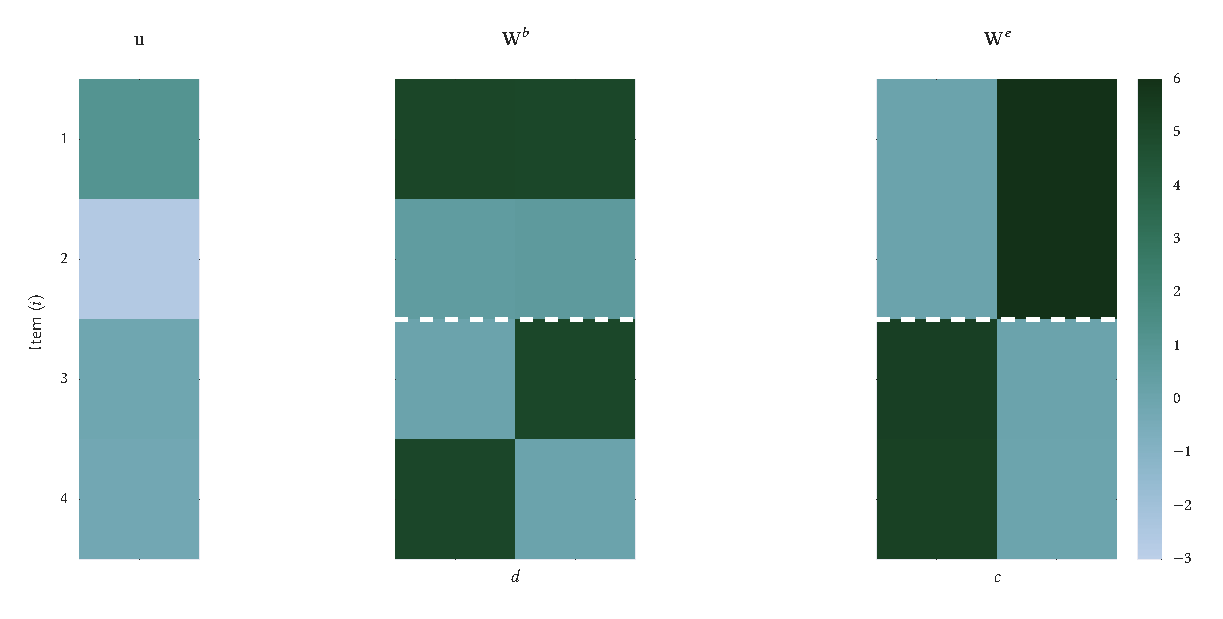
\includegraphics[width=\textwidth]{fldc_toy_example_learned_weights}
  \caption{Learned model for example \ref{sec:fldc-toy}. The white line divides the disjoint pairs described in the example.}
  \label{fig:fldc-toy-learned-weights}
\end{figure}

The model shown in the figure displays the desired properties of diversity between the disjoint pairs whilist having coherence between the items in each pair. Despite being different from the proposed model in section \ref{sec:fldc-toy} it approximately realizes the desired distribution.

\subsubsection{FFLDC: Rated locations}

Firstly, recall the following characteristics about the dataset in the example:

\begin{itemize}
  \item There are 6 items, i.e. $V = \{1,2,3,4,5,6\}$.
  \item The full distribution is related to the features and is given in table \ref{tab:ffldc-toy-probs}.
  \item The proposed model has 2 diversity dimensions and one coherence dimension.
\end{itemize}

\begin{figure}
  \centering
  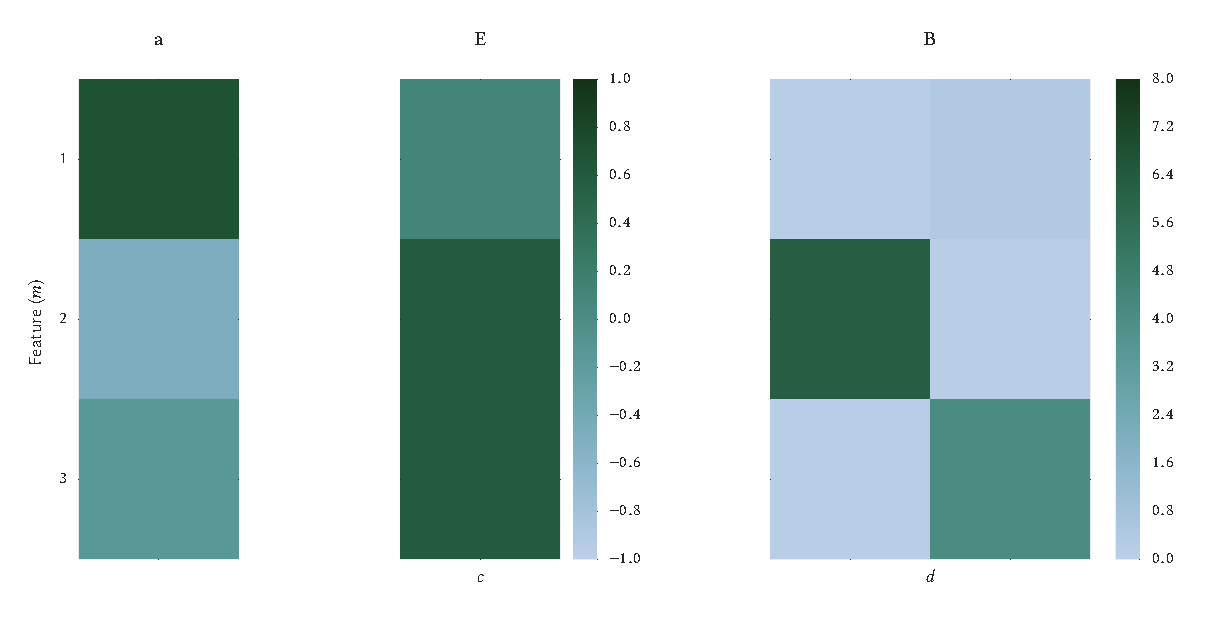
\includegraphics[width=\textwidth]{ffldc_toy_example_learned_weights}
  \caption{Learned model for example \ref{sec:ffldc-toy}}
  \label{fig:ffldc-toy-learned-weights}
\end{figure}

Figure \ref{fig:ffldc-toy-learned-weights} shows the resulting model after learning. Unfortunately, this model can be not as easily interpreted as the one proposed in figure \ref{fig:ffldc-toy-all-weights}, nevertheless it accurately models the distribution from the example. This result demonstrates the ability of the learning algorithm to represent a distribution using features.

It is important to note that the presented results for these experiments correspond to the best of multiple runs. It was observed that the learning algorithm does not always arrive to a good solution. This is explained by the fact that $g(\theta)$ is not a convex function which means that there exists the risk of reaching a local minima in some cases. Due to this, most of the experiments in the following sections are executed over several data folds to account for the randomness.

\subsection{Adagrad}
\label{sec:adagrad}

This section will introduce a modification to the SGD method which was found to be useful when dealing with real data and featurized models.

A commonly used learning rate function for SGD is $\eta(t) = \eta_{0}t^{-p}$, which offers the best convergence speed in theory and also does it often in practice \citep{bottou2012stochastic}, however it can also lead to poor performance due to slow rates of convergence to the solution \citep{darken1992towards}. On the other hand choosing a larger $\eta_{0}$ may not lead to better results due to the instability in the parameters for small $t$ \citep{Darken1990}. 

This behavior was observed during the experiments with real data to be presented in later sections, therefore an alternative for the learning rate was sought. In particular, Adaptive Gradient (AdaGrad) was implemented.

AdaGrad was proposed by \citet{Duchi2011adagrad}, the idea of this method is to adapt the learning rate for each parameter in $\theta$ individually in a way that frequently updated parameters have slower learning rates while infrequent parameters have larger ones. The intuition is that an update to a rare parameter is more informative than one to a parameter that is frequently updated.

Concretely, with AdaGrad the update step for each parameter in $\theta$ is given by:

\begin{equation}
  \theta^{\tau + 1}_{j} \leftarrow \theta^{\tau}_{j} - \frac{\eta}{\sqrt{G_{j,j}}} \nabla g(\theta)^{\tau}_{j}
\end{equation}

Where $G_{j,j}$ contains the information about past gradients for parameter $j$ and is given by:

\begin{equation}
  G_{j,j} = \sum_{t=1}^{\tau} \left(\nabla g(\theta)^{t}_{j}\right)^{2}
  \label{eq:adagrad-g}
\end{equation}

In equation \ref{eq:adagrad-g} $\nabla g(\theta)^{t}_{j}$ denotes the $j$-th entry of the gradient at time step $t$.

It is worth noting that AdaGrad does not incur in an significant increase in running time or memory requirements for the training which makes it inexpensive to include in the implementation of NCE.

\subsection{Learning rate sensitivity}

This section expands on the discussion about the learning rate and explores its effect on the learning of the synthetic data from the FFLDC example in section \ref{sec:ffldc-toy}, as well as the effect of implementing AdaGrad.

The first experiment considers the stability of the optimization without AdaGrad. In the experiments presented in this section the following configuration of the learning algorithm is used:

\begin{itemize}
  \item 1000 data samples from the distribution in table \ref{tab:ffldc-toy-probs} are used, along with 2000 noise samples, i.e. $\nu = 2$.
  \item Each run does 100 passes over the data and noise samples.
  \item The algorithm is executed 8 times to obtain statistics about the results.
\end{itemize}

Figure \ref{fig:effects_eta_0} shows the behavior of $g(\theta)$ during learning, each point corresponds to the average value of $g(\theta)$ after each pass over the data and noise samples with its corresponding 95\% confidence interval.

\begin{figure}
  \centering
  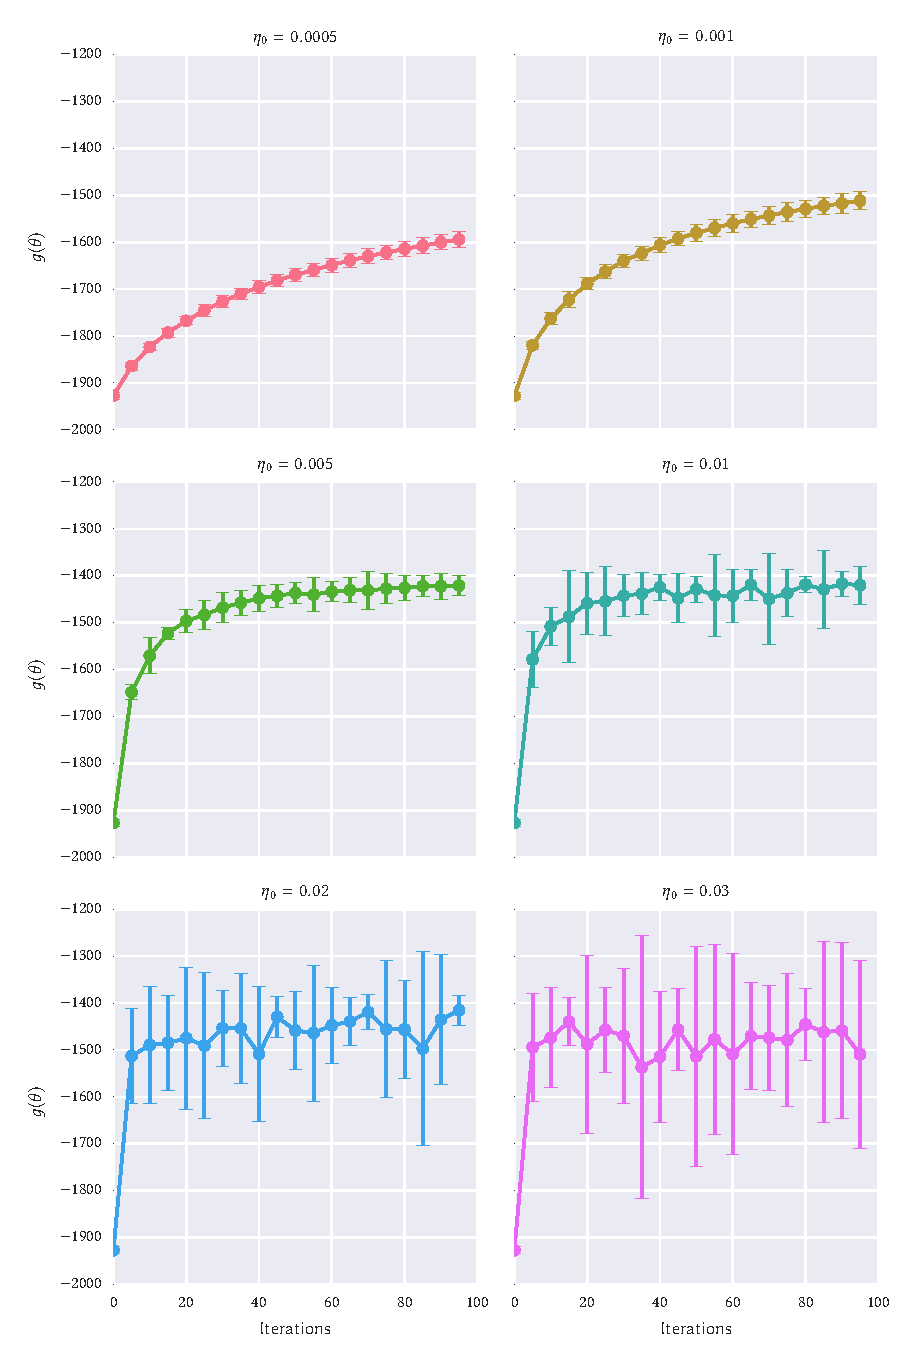
\includegraphics[width=\textwidth]{effects_eta_0_ffldc}
  \caption{Objective function during learning for various values of $\eta_0$ without AdaGrad.}
  \label{fig:effects_eta_0}
\end{figure}

The results in figure \ref{fig:effects_eta_0} display what was mentioned in section \ref{sec:adagrad}, they show that for small values of $\eta_0$ the learning can be significantly slow and that large values of $\eta_0$ may lead to instability. Concretely,  the first row displays slow but stable learning rates while the last row displays learning rates that are too high, the middle row displays the ideal learning rates. Fortunately, in the particular case of this synthetic dataset there exists a learning rate for which the objective function converges however, as it will be seen on real data, this is not always the case. An interesting characteristic shown in this figure is the behavior of the confidence intervals for $\eta_0 = 0.005$, even though the learning is considerably slow there is also a large variation, in this instance the initialization has a larger influence because the learned model doesn't change much from it.

In contrast, figure \ref{fig:effects_adagrad} shows the objective function for various values of $\eta_{0}$ after incorporating AdaGrad to the implementations. These results show that training with AdaGrad is stable for a larger range of $eta_0$, although slower for small values of $\eta_{0}$ which were good for the learning without AdaGrad. For large enough $\eta_0$ values, it can be clearly seen from the figure that SGD with AdaGrad reaches convergence significantly faster, often in the first few iterations.

\begin{figure}
  \centering
  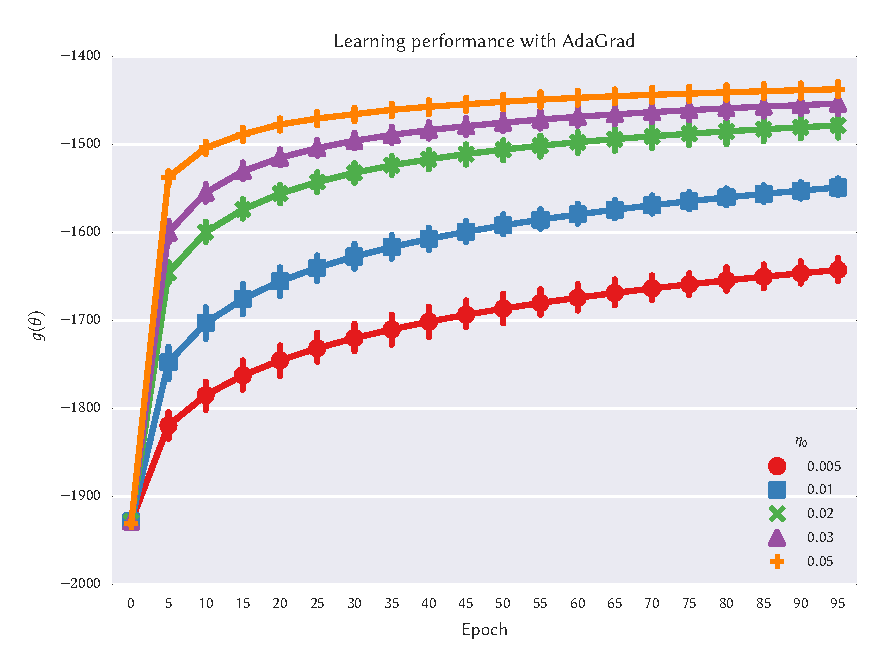
\includegraphics[width=\textwidth]{effects_eta_0_ffldc_adagrad}
  \caption{Objective function during learning for various values of $\eta_0$ with AdaGrad.}
  \label{fig:effects_adagrad}
\end{figure}

Finally, figure \ref{fig:comparison_adagrad_ffldc_toy} shows a direct comparison between training with and without AdaGrad using the best values of $\eta_0$ for each configuration. In this figure both algorithms converge to an optimal value, however it also shows that training with AdaGrad converges significantly faster and its average appears slightly more stable.

These combined results indicate that using AdaGrad is the best strategy for learning the models.

\begin{figure}
  \centering
  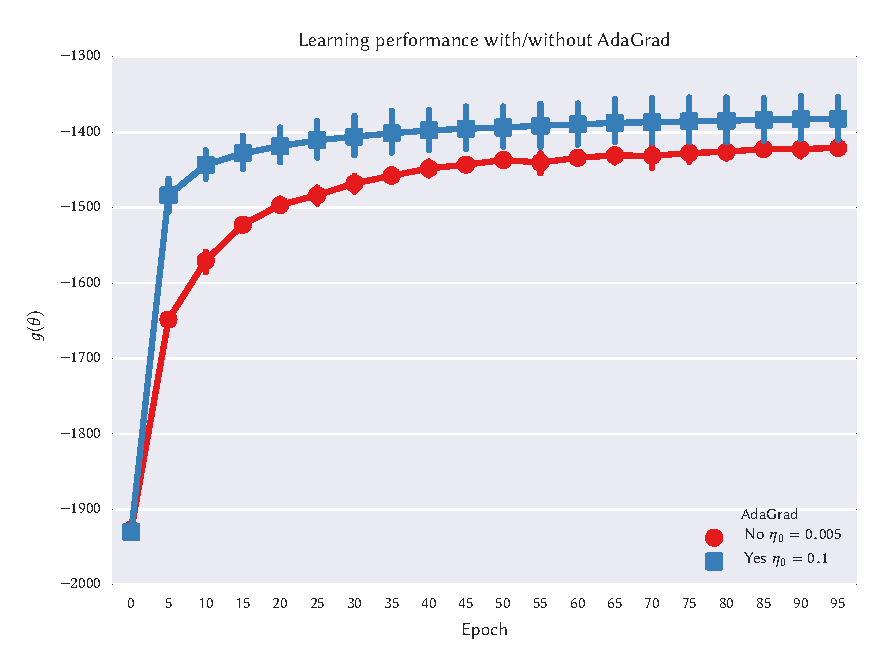
\includegraphics[width=\textwidth]{ffldc_adagrad_comparison}
  \caption{Comparison of learning performance with and without AdaGrad. Initial learning rates are $\eta_0 = 0.05$ with AdaGrad and $\eta_0 = 0.005$ without AdaGrad.}
  \label{fig:comparison_adagrad_ffldc_toy}
\end{figure}

\subsection{Noise-to-data ratio}

One final consideration about NCE is how to choose the noise, \citet{Gutmann12NCE} suggest the following about the noise distribution:

\begin{itemize}
  \item A distribution that can be sampled easily.
  \item Noise that is as similar as possible to the data, otherwise the classification problem could be too easy.
  \item A noise sample as large as possible.
\end{itemize}

Following the first two suggestions, the noise distribution is sampled from a modular model as the one from equation \ref{eq:modular}. This distribution is constructed from estimated marginals, i.e. $\hat{P}(i \in S)$, which are computed using the maximum likelihood estimator, i.e. $\hat{P}(i \in S) = \nicefrac{\#N(i \in S)}{|\mathcal{D}|}$. Then the utilities for the modular model are given by:

\begin{equation}
  u_{i} = \log{\left(\frac{1}{\hat{P}(i \in S)} - 1\right)}
\end{equation}

This model is easy to sample from, hence allowing an efficient generation of large noise samples.